\documentclass[a4paper,10pt]{article}          % LaTeX 2e 
%, twocolumn

\usepackage{ae}
\usepackage{multicol}
\usepackage[left=2cm,right=2cm,top=2cm,bottom=2.5cm]{geometry}

%\usepackage[german]{babel}

\usepackage[T1]{fontenc}

\usepackage{ifthen}
\usepackage{graphicx}
\usepackage{longtable}

\usepackage{enumitem}
\usepackage{listings}
\usepackage{color}

\clubpenalty=10000
\widowpenalty=10000
\displaywidowpenalty=10000 


\def\textfraction{0.01}
\def\topfraction{0.99}
\def\figscale{0.6}

\renewcommand{\baselinestretch}{.98 }

\newcommand{\code}[1]{{\ttfamily#1}}

%\pagestyle{empty}

\title{GreenSocket - Conceptual Details}

\author{\sffamily{Robert G\"unzel (GreenSocs)}}

\date{}



	\lstset{language=SystemC, %Syntax Higlight
		basicstyle=\scriptsize, 
		identifierstyle=\ttfamily,
		commentstyle= \color[rgb]{0,0.5,0} \ttfamily, 
		stringstyle=\color[rgb]{0.7,0,0} \ttfamily,
		keywordstyle=\color[rgb]{0,0,.8} \ttfamily,
		showstringspaces=false,
		numbers=left,
		numberstyle=\tiny,
		stepnumber=1,
		numbersep=5pt, 
		captionpos=b,
		frame= {tblr},
		basewidth={0.5em,0.45em}
		} 
	\lstset{escapeinside={(*@}{@*)}} % To add labels in listing, needs own line

\begin{document}



\maketitle

\begin{abstract}
This document describes the basic concepts used within greensocket. It tries to give reason for some decisions, and explains some non-trivial things within the code. You should first read this document, and then look into the code and its documentation. Starting with looking at the code can cause bad headache. Btw: When I say "In-code documentation" this could be interpreted as "documentation or the code itself", because sometimes code is more expressive than a hundred words written by non-native English speakers. But I am currently in the process of improving the quantity and quality of the available in-code documentation.
\end{abstract}

\section{Initiator Socket}

The class hierarchy of the initiator socket is shown in figure \ref{fig:isockch}.

\begin{figure}[htbp]
\begin{center}
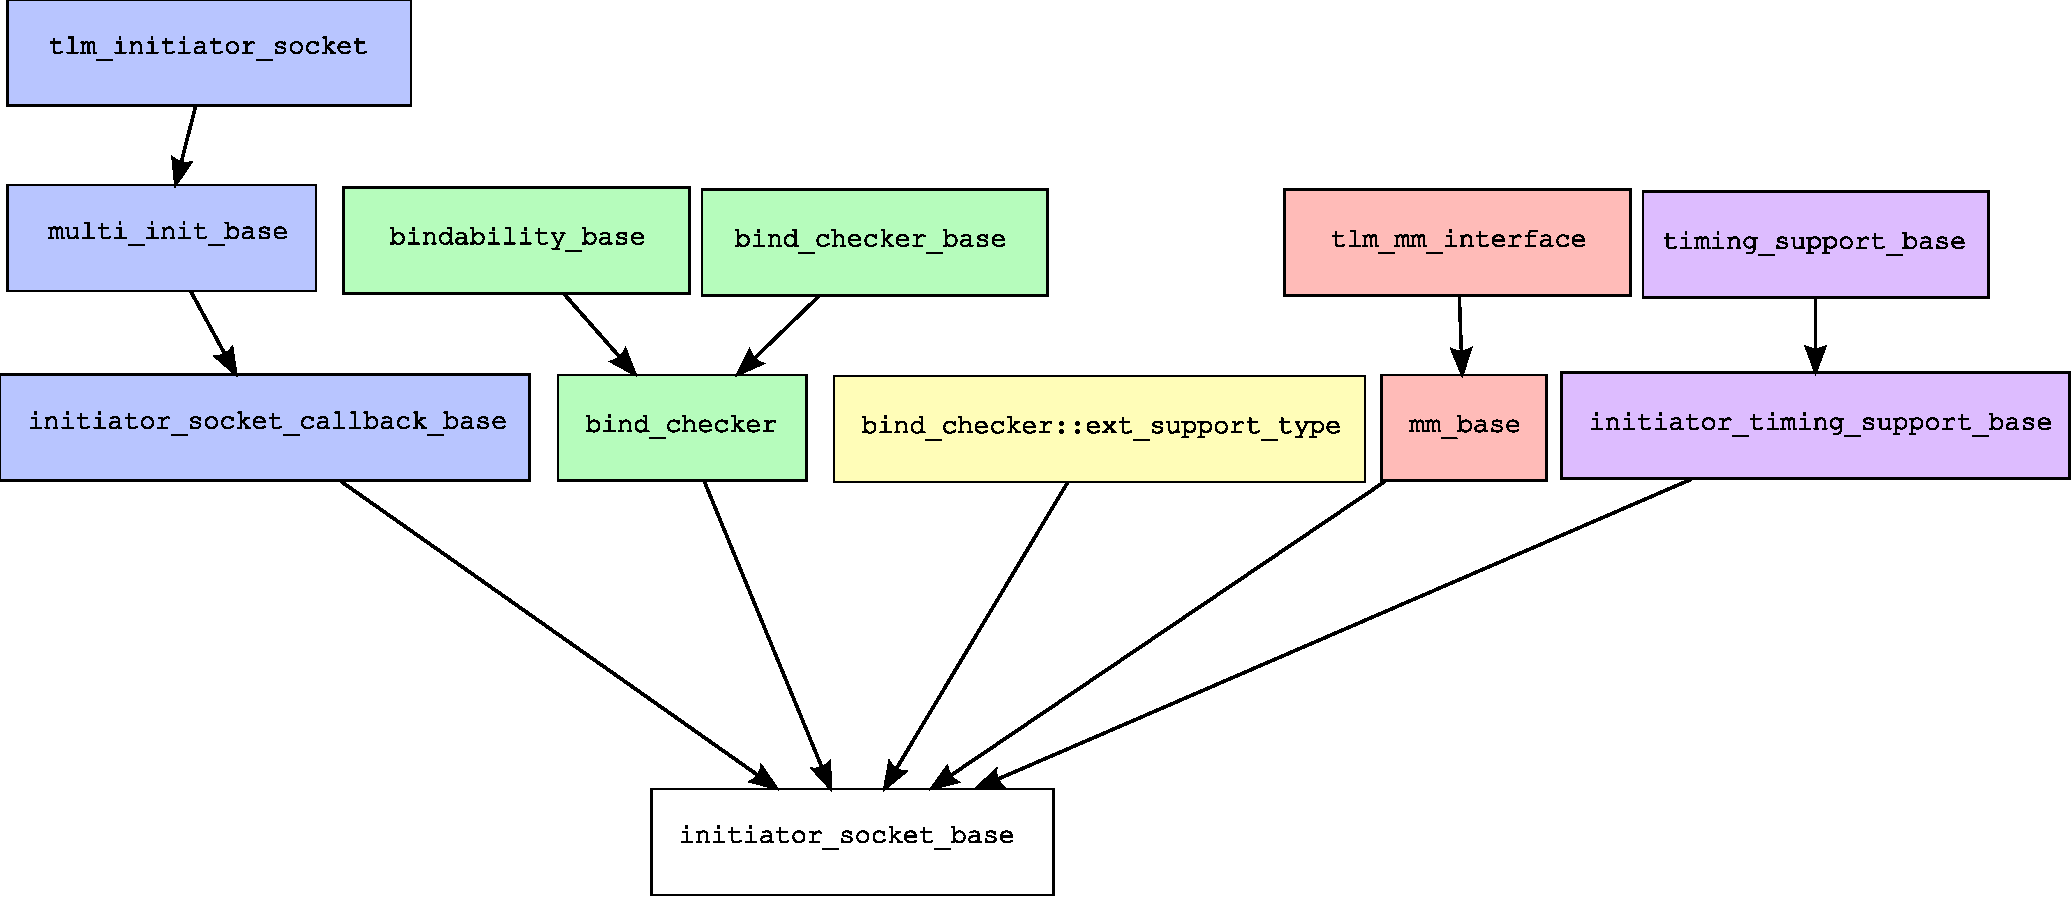
\includegraphics[scale=0.4]{isockch}
\caption{Initiator Socket Class Hierarchy}
\label{fig:isockch}
\end{center}
\end{figure}

It can be seen that the initiator socket is founded on five "pillars": the actual \code{tlm\_socket} (blue), the runtime bind check facilities (green), the extension support API (yellow), the memory management facilities (red), and the timing information distribution support facilities (purple).

The \code{initiator\_socket\_base} (white) is just the glue to connect the five pillars. The class is defined as:

\begin{lstlisting}
template <unsigned int BUSWIDTH=32,
          typename TRAITS=tlm::tlm_base_protocol_types,
          unsigned int N=0,
          typename BIND_BASE=bind_checker<TRAITS>,
          typename MM_INTERFACE=tlm::tlm_mm_interface,
          typename EXT_FILLER=mm_base<TRAITS,MM_INTERFACE>,
          typename POOL=default_pool<TRAITS, EXT_FILLER>
          >
class initiator_socket_base: 
                              public initiator_socket_callback_base<BUSWIDTH,TRAITS, N, 
                                                                    typename BIND_BASE::root_type, 
                                                                    typename BIND_BASE::multi_root_type>
                            , public BIND_BASE
                            , public BIND_BASE::ext_support_type
                            , public mm_base<TRAITS,MM_INTERFACE>
                            , public initiator_timing_support_base<TRAITS,BIND_BASE>
{
...
initiator_socket_base(const char* name, allocation_scheme alloc_scheme=mm_txn_only(), EXT_FILLER* ext_filler=NULL);
...
};

\end{lstlisting}

Obviously some of the base classes of the \code{initiator\_socket\_base} are defined by template arguments of the class, defaulting to the classes shown in figure \ref{fig:isockch}. Let's quickly go through the set of template arguments:

\begin{description}
\item[\code{int BUSWIDTH}]:

Nothing to say here, I guess. Read the TLM-2.0 LRM, in case you do not know.
\item[\code{typename TRAITS}]:  

Defines the type of the used transaction and phase type. Again, have a look into the TLM-2.0 LRM, in case you don't know how that is supposed to work.

\item[\code{int N}]:

Defines the number of allowed bindings for a greensocket in a similar way as it is done for \code{sc\_port}s. That means, if N=0, an unlimited number of bindings are allowed, if N=X exactly N bindings are required.

\item[\code{typename BIND\_BASE}]: 

That class is the foundry for the runtime bind checks in greensocket. Its default can be used as long as the transaction type within the traits class has an extension mechanism with an API identical to the one of the TLM generic payload. If that is not the case, you will have to use a custom bind checker, whose bind checks are not extension based. As you can see in line 10 and 11 the bind checker needs to provide some typedefs that are used within the TLM socket pillar of the greensocket. The reason for that is that the bind checks are performed using dynamic casts, so to this end the bind checker needs to define some classes that are used in the TLM socket pillar of the greensocket. Replacing the bind checker is a non-trivial task, but as long as you use the generic payload and the TLM phase type, you'll never have to do that. Accept that as an experimental feature only the developer of greensocket (which would be me) can use. So in case I die that feature dies with me. So just ignore it. Really.

\item[\code{typename MM\_INTERFACE}]:

That class is used as the base of the \code{mm\_base} class. It is the memory management interface of the payload you are using. In case of the generic payload, this is the \code{tlm\_mm\_interface} (the default here). But if you use a different payload (even if it is compatible with the bind checker, i.e. it has the same extension API as the generic payload), you need to provide a new  memory management interface class, as the type of the payload is fixed to the generic payload in the \code{tlm\_mm\_interface}. The restriction here is that the provided class should only contain a single function named \code{free}, returning \code{void} and taking a pointer to your payload type (compare it to the \code{tlm\_mm\_interface}). The purpose of this class is described in the TLM-2.0 LRM.

\item[\code{typename EXT\_FILLER}]:

That class should contain a function named \code{fill\_txn} taking a ptr to your payload type as an argument and returning a pointer to your payload type as well. The name comes from the fact that the \code{fill\_txn} function is supposed to pre-fill a transaction with extensions before it is put into the pool.

You can see that a pointer to an instance of such an extension filler is passed as a CTOR argument to the socket (line 19), and it defaults to \code{NULL}. The rule here is that if you leave that argument \code{NULL} the socket will use \textbf{itself} as an extension filler. Of course that does only work if you did not provide your own extension filler class, because in the default case the extension filler in use is the \code{mm\_base} class, and the socket is always derived from that class (see line 15), and hence can really use itself as an extension filler.

If you use your own extension filler type you have to provide a pointer to an instance of it as the ctor argument. Note that if you define your own extension filler class and set the template argument to it and you DO NOT set the ctor arg, you will most likely run into a seg fault. You should take that as an experimental feature.

\item[\code{typename POOL}]:

Allows to define the class that is used as a pool. Initially I thought it might be nice to let people choose what kind of pool they wanna use, but frankly never ever was there a user of greensocket who wanted to use another pool. So basically, this template argument should never be changed. During the evolution of greensocket the pool became more and more tightly coupled to the rest of the code. It is not recommended to try to replace it. The default pool uses the aforementioned extension filler to initialize transactions before they go into the pool. Note that it does that only when the transaction is first added to the pool. Not everytime something returns to the pool. It is meant to do once-in-a-lifetime things like adding sticky extensions, allocating data arrays, etc.

\end{description}
 
Now in some places a virtual interface might seem more appropriate than the template stuff I am doing. The reason is that I wanted to avoid virtual calls to avoid the overhead of the vtable look ups (especially in the high speed LT use case) for accesses to the pool, the extension filler or the extension API. So I needed to know the actual class name (via a template arg) instead of just some virtual base class type.

To illustrate that the flexibility sketched above really exists (even including the experimental features) take a look at the code below. It shows a greensocket that is fully customized (i.e. all template args are overridden, apart from the POOL template arg).

\begin{lstlisting}
/*
 *  Created by Robert Günzel on 27.05.08.
 *  Copyright 2008 E.I.S.. All rights reserved.
 *
 */

#include "greensocket/initiator/single_socket.h"
#include "greensocket/target/single_socket.h"

struct my_payload; //fwd declaration so that we can define the mm interface


//mm interface in its must have structure
struct my_mm_interface{
  virtual void free(my_payload*)=0;
  virtual ~my_mm_interface(){}
};


//minimum example of custom payload
struct my_payload{

  //the mm functions must be there
  void acquire(){assert(m_mm != 0); m_ref_count++;}
  void release(){assert(m_mm != 0); if (--m_ref_count==0) m_mm->free(this);}
  int get_ref_count(){return m_ref_count;}
  void set_mm(my_mm_interface* mm) { m_mm = mm; }
  bool has_mm() { return m_mm != 0; }

  //reset must be there
  void reset(){}

  //mm_interface ptr and ref count must be set up properly
  my_payload(): m_mm(NULL), m_ref_count(0){}
  
  //mm_interface ptr and ref count members must be there
  my_mm_interface* m_mm;
  unsigned int m_ref_count;
};

//minimum example of custom phase
struct my_phase{};

//custom traits class
struct my_traits{
  typedef my_payload tlm_payload_type;
  typedef my_phase   tlm_phase_type;
};

//minimum example of custom bind check classes
class my_bind_base{}; //this class is normally used for dynamic casts and exchanging configs
class my_config{};    //this class would normally contain your custom configuration structure that is compared during bind
class my_ext_supp     //this class would normally contain getters and setters for your extensions
{
public:
  virtual ~my_ext_supp(){} //class needs to be polymorphic  
  my_ext_supp(unsigned int){std::cout<<"nothing at ALL!!!!!"<<std::endl;} //this ctor must be there
};

//this class is responsible for filling txns before they go into the pool
class my_ext_filler
{
public:
  my_ext_filler():test(NULL){}

  my_payload* fill_txn(my_payload* t){ //fill txn must set mm ptr
    if (!test) std::cout<<"damn"<<std::endl;
    else t->set_mm(test);
    std::cout<<"I don't fill anything..."<<std::endl;
    return t;
  }
  
  my_mm_interface* test;
  
};

//bind checker must be derived from bind_base
class my_bind_checker:
public my_bind_base
{
public:

  //this function must be there (normally it should handle the dynamic bind checking)
  // it would now need to get a ptr to the connected other side (the uint tells which connection
  // of the underlying socket). It can then cast it into bind_base, then get the config of the
  // other side and finally compare it
  void check_binding(unsigned int){std::cout<<"I do not check bindings. The traits class is good enough!"<<std::endl;} 
  
  //this ctor must be there (provides name and pointer to owning socket (as void))
  my_bind_checker(const char* name, void*){
    std::cout<<name<<" bind checker ctor empty!!!!!"<<std::endl;
  }
  
  //those type defs must be there
  typedef my_bind_base       bind_base_type;
  typedef my_config           config_type;
  typedef my_ext_supp        ext_support_type;
  typedef gs::socket::gs_callback_binder_base             root_type;
  typedef gs::socket::gs_multi_to_multi_bind_base<my_traits> multi_root_type;
};

SC_MODULE(Master){

  //a socket with custom traits and custom bind_checker and custom mm_interface and custom ext_filler
  // (you only need custom bind_checker and custom mm_interface and custom ext_filler if your custom
  // traits class does not contain the generic payload)
  
  my_ext_filler m_ext_fill;
  typedef gs::socket::initiator_socket<32, my_traits, my_bind_checker, my_mm_interface, my_ext_filler> i_sock_type;

  i_sock_type socket;
  
  SC_HAS_PROCESS(Master);
  Master(sc_core::sc_module_name name, bool dyn): sc_core::sc_module(name), 
          socket("socket",i_sock_type::mm_txn_with_data(),&m_ext_fill)
  {
    m_ext_fill.test=&socket;
    SC_THREAD(run);
  }

  void run(){
    wait(10,sc_core::SC_NS);
    my_payload* p=socket.get_transaction();
    my_phase ph;
    sc_core::sc_time t;
    socket->nb_transport_fw(*p,ph,t);
  }
};

SC_MODULE(Slave){
  typedef gs::socket::target_socket<32, my_traits, my_bind_checker> t_sock_type;

  t_sock_type socket;

  SC_CTOR(Slave): socket("socket")
  {
    socket.register_nb_transport_fw(this, &Slave::trans);
  }

  tlm::tlm_sync_enum trans(my_payload&, my_phase&, sc_core::sc_time&){
    std::cout<<"FOO"<<std::endl;
    return tlm::TLM_ACCEPTED;
  }
};



int main(int, char** argv){
  Master m("m", true);
  Slave  s("s");
  m.socket(s.socket);
  sc_core::sc_start();
  return 0;
}
\end{lstlisting}

You can see that the greensocket is fully customized. It now uses a custom payload, a custom phase, and a custom bind check mechanism. The bind check mechanism is not actually performing a check. It relies on the compiled time bind check defined by TLM-2.0. Since it does not use extensions the extension support class is empty.

So what is actually left of greensocket is merely that you can use a pool, and that you have a tagged multi socket. But as soon as you stick with the generic payload, it also offers a special extension API, runtime bind checks and appropriate socket configurability.

Now the different pillars will be investigated.

\subsection{TLM Socket}

As can be seen in figure \ref{fig:isockch}, the socket pillar is founded on the \code{tlm\_initiator\_socket}.  What is added on top of it? Functionally, it is the ability to register callbacks and to enable sender identification when the socket is bound multiple times.
What does "sender identification" mean.

Let's assume you bound your initiator socket two times (to two distinct targets). Now if you do \code{socket[0]->nb\_transport\_fw(...)} it will arrive at the target socket bound at index 0. And if you code{socket[1]->nb\_transport\_fw(...)}  it will arrive at the target socket bound at index 1. So far so good. But you only have one socket. So you will register only one callback (e.g. \code{nb\_transport\_bw}). Now if one of the targets calls \code{nb\_transport\_bw} on its socket, it should end up at your initiator. But usually you wanna know which target just talked to you. So the callback should not only pass the payload, phase and time to you, but also the index of the connection over which the call came in. That means if you get \code{nb\_transport\_bw} with index=x, then you will reach the target that called you via \code{socket[x]->nb\_transport\_fw(...)}.

Such a functionality is available in the multi-passthrough-sockets of the TLM-2.0 utils, but unfortunately they lack some features requested by greensocs users (mainly adding a tag on top of the sender identification), and the class structure does not allow for runtime bind checks (they are lacking some mechanisms to navigate safely through the module hierarchy).

So the TLM socket pillar does that.  But how does that work?

First let's discuss the basic idea. 


\begin{figure}[htbp]
\begin{center}
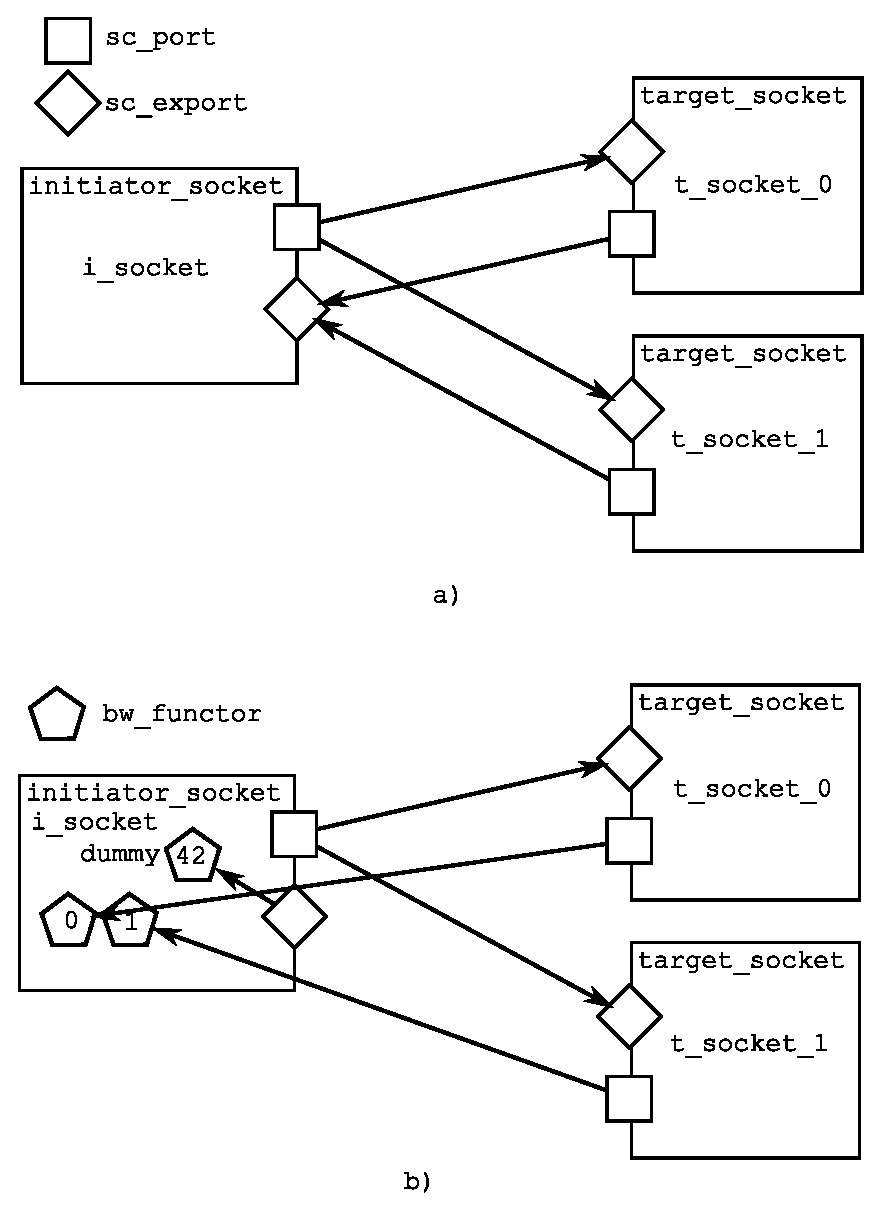
\includegraphics[scale=0.7]{multib1}
\caption{Multi-bind situation sktech 1}
\label{fig:multib1}
\end{center}
\end{figure}

Consider the setup shown in figure \ref{fig:multib1}a. There you can see a plain TLM initiator socket named \code{i\_socket} that is bound to two target sockets. Now you may call \code{i\_socket[0]->nb\_transport\_fw} or  \code{i\_socket[1]->nb\_transport\_fw} two decide to talk to which target. However, there is a problem to that, which will hurt us later in the process: Let's assume you first bind \code{t\_socket\_0} and then \code{t\_socket\_1}, then you would expect that the call to  \code{i\_socket[0]->nb\_transport\_fw} will end up at \code{t\_socket\_0}. But the SystemC standard explicitly states that you cannot make such an assumption. The binding sequence does not necessarily reflect the order in the underlying data structure that is accessed via the \code{operator []}. Keep that in mind. We will come to that later.

Now if one of the target sockets are used like that \code{t\_socket\_1->nb\_transport\_bw} it will call the interface bound to the export of the initiator socket. Since only one interface can be bound to an export it will be impossible to distinguish between the actual caller of \code{nb\_transport\_bw}. 

The basic concept of identifying the caller is shown in \ref{fig:multib1}b.
When the initiator socket is bound to a target, we will bind the initiator sockets export to a dummy interface (so that SystemC doesn't complain about an unbound export), and then we will bind the port of the target socket to a functor object (within greensocket we call that functor a binder, because we bind it to a port). Such a functor has an internal ID, starting at zero and being incremented with every binding. Then the functor can add this ID when performing a callback into the owner of the initiator socket, so the owner can distinguish between different callers of \code{nb\_transport\_bw} (or other bw calls). Note that the dummy interface is a functor as well. In greensocket it has ID=42. So whenever you face an error and the binder ID is 42, you somehow ended up at the dummy.

Now we can identify the sender, but remember the problem with the \code{operator []} I mentioned above. The bw calls now have an ID that reflects the target bind orders. In other words (as I said already) the second target that was bound will always have ID 1, and the third target will have ID 2, and so on. But that is not necessarily the index I need to use in the \code{operator []} of the \code{sc\_port} to reach the target. So, we need to make sure that works.

Figure \ref{fig:multib2} shows, how that is done. When the initiator socket is bound, we first bind the \code{sc\_port}, so that it can be used to track the correct number of bindings and used binding policy, but we will not use it for communication actually. Instead during the bind, we get a pointer to the forward interface (the interface bound to the export) of the target socket, and put it into a data structure whose index reflects the binding sequence (a vector). Then we override the \code{operator []} of the initiator socket, so that it does not use the operator of the underlying \code{sc\_port}. Instead the operator will just return the interface from our own internal vector. By doing that, both the \code{operator []} and the IDs added to the backward calls will reflect the binding sequence, so that we can be sure that a caller who is identified with \code{ID=x}, can be reached via \code{i\_socket[x]->nb\_transport\_fw}.

\begin{figure}[htbp]
\begin{center}
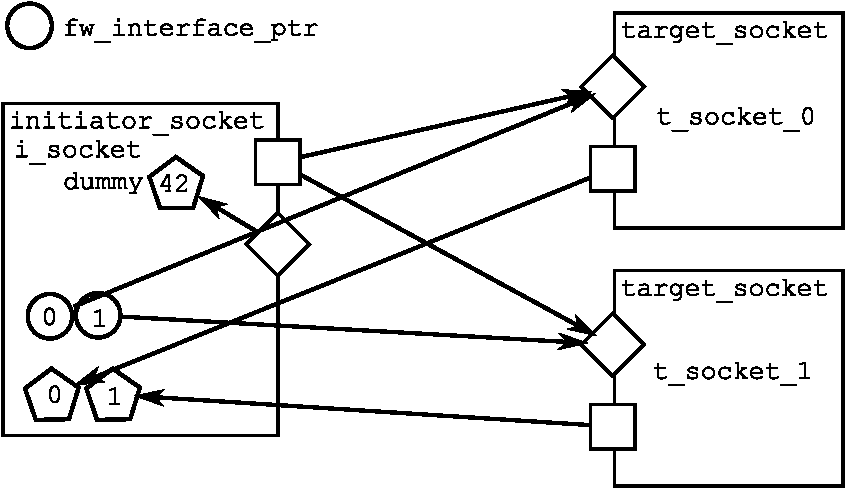
\includegraphics[scale=0.7]{multib2}
\caption{Multi-bind situation sktech 2}
\label{fig:multib2}
\end{center}
\end{figure}

Now, let's look at some special things. Have a look at the class definition of the \code{initiator\_callback\_base}


\begin{lstlisting}
template <unsigned int BUSWIDTH = 32,
          typename TRAITS = tlm::tlm_base_protocol_types,
          unsigned int N=0,
          typename CB_BINDER_BASE=gs_callback_binder_base,
          typename MULTI_MULTI_BASE = gs_multi_to_multi_bind_base<TRAITS>
          >
class initiator_socket_callback_base: public multi_init_base< BUSWIDTH, 
                                                        TRAITS,
                                                        N,
                                                        CB_BINDER_BASE
                                                        >
{
...
  template <typename T>
  initiator_socket_callback_base(const char* name, T* owner);
...
};
\end{lstlisting}

Again, we see a disgustingly large number of template arguments. The first three are inevitable because of TLM-2.0, but what do the other two stand for?

\begin{description}
\item[\code{CB\_BINDER\_BASE}]:

This class is used as the very base of the binder objects (the functors used to bind the ports). This class has to provide the following functions and members:
\begin{lstlisting}
public:
    int get_index(); //return ID
    void* get_owner(); //return ptr to socket owner
    template<typename T>
    void  set_owner(T* owner); //set ptr to socket owner
    void set_offset(unsigned int offset); //set tag offset
    template<typename T>
    /*constructor*/(int id, T* owner, unsigned int offset);
protected:
    void* m_owner;
    unsigned int m_id;
    unsigned int m_offset;  
\end{lstlisting}

This is pretty precise, so why is that a template? That has political reasons. We have projects where the bind check mechanism was enhanced by user requests. In such cases the whole bind checking facilities were licensed to the customers (i.e. not open source) while the rest of greensocket remained unchanged and open source. However, the bind checkers need the binder base class to do dynamic casts and stuff. So they basically belong to the closed source part. So we needed a mechanism that allows to replace this binder base class. So we use a template argument for that.

Note that the owner is used as a void pointer. How is that supposed to work? The ctor in lines 14 and 15 of the class definition show that owner is actually passed to the \code{initiator\_socket\_callback\_base} as some type \code{T}. This pointer is then re-interpreted into a void pointer (i.e. without any application of offsets). Now, what \code{T} is that? The \code{initiator\_socket\_base} calls the ctor of the \code{initiator\_socket\_callback\_base} like that:

\lstinline{initiator_socket_callback_base(name, static_cast<typename BIND_BASE::bind_base_type*>(this))}

Maybe you remember that the \code{BIND\_BASE} template arg of the \code{initiator\_socket\_base} was the class that is used to define the bind checking facilities. That means that the initiator passes itself (as some type defined in the \code{BIND\_BASE} class) to the \code{initiator\_socket\_callback\_base}. The \code{initiator\_socket\_callback\_base} will then re-interpret that pointer into void and give it to the binder base class. As mentioned before only the bind facility needs the owner pointer. So it can just get the void pointer and re-interpret it again as the type it knows (\code{bind\_base\_type}). Of course the prerequisite here is that the bind facility is derived from this type.  

\item[\code{MULTI\_MULTI\_BASE}]: 

When two multi sockets (a multi initiator and a multi target) are bound, the initiator must be able to detect that. Because in that case it cannot simply put the interface of the export of the target into its set of bound interfaces. It needs to ask the multi target for the corresponding binder interface (because the export of the multi target will be bound to a dummy interface, just like the initiator). The initiators can check this using a dynamic cast into the \code{MULTI\_MULTI\_BASE} class. Again, why is this a template argument? Politics again. The multi sockets that are part of TLM-2.0 use just the same concept to support multi binds (which is no suprise, as I have written them as well). So basically we could have used the multi-to-multi-bind-base from TLM-2.0 for greensocket, but the SystemC license is by far too restrictive. So we have our own class with our own license (since the copyrights remain at the contributor, which is GreenSocs, we can legally do that). But that means greensockets cannot be bound to multi sockets of TLM-2.0 directly. You can either insert a flange (a module that has a target and an initiator socket and that directly forwards stuff from one side to the other), or you replace this template arg with the TLM-2.0 multi base (you can do that by defining your own bind checker, e.g. by deriving from the greensocket bind checker, and replace the \code{multi\_root\_type}. Then use this bind checker for the greensocket).
 
\end{description}

Okay. Now, what is the \code{multi\_init\_base} for? It is just a virtual interface class that clearly defines the interface between hierarchically bound init sockets. That's all.

Finally, one more important note: In first versions greensocket existed in a single and a multi socket version. The single version did not use binders or anything, because it is not needed. However, maintaining two separate sockets is a pain, so we decided that we can drop the single socket as it is functionally a subset (a multi socket that is just bound once) of multi sockets. Unfortunately, you then end up getting always the ID=0 added to your callbacks, although you are not at all interested in it, as you know the thing is only bound once. And the single socket is by far the more common case (one bus model with multi sockets $\Rightarrow$ one hundred IP models with single sockets).

So, we added the feature that the callback signatures used by the greensockets change when the template argument \code{N} is set to one. That involves some more template meta programming, but does not change the overall concept. This feature is (or will be) documented in the code.

Another note: the support for hierarchical bindings is described in code as well.

\subsection{Bind Checking}

Here I will describe the bind checking employed by greensocket in the default case. This section might be a good starting point if you intend to write your own bind checker.

\subsubsection{Base classes}

The bind checker has two base classes:

\begin{lstlisting}
template <typename TRAITS>
class bindability_base{
public:
  virtual gs::socket::config<TRAITS>&       get_config(unsigned int)=0;
  virtual bool get_t_piece_end(bindability_base*&, unsigned int&)=0;
  virtual const char* get_name()const =0;
  virtual sc_core::sc_object* get_parent() =0;
  virtual ~bindability_base(){}
};


template <typename TRAITS>
class bind_checker_base
{
public:
  virtual void set_config(const gs::socket::config<TRAITS>&)=0;
  virtual void set_config(const gs::socket::config<TRAITS>&, unsigned int)=0;
  virtual gs::socket::config<TRAITS>& get_recent_config(unsigned int index=0)=0;
  virtual ~bind_checker_base(){}
};
\end{lstlisting}

The \code{bindability\_base} is the interface used between an initiator and a target socket during their bind check. The \code{bind\_checker\_base} is the interface between the user of a socket and the socket's bind check facility. The purpose of the various functions is described in code. Their names a good enough for this document. The only thing that may seem weird is the \code{get\_t\_piece\_end}. What is a T-piece? 

A T-piece is a module with exactly one target greensocket and one initiator greensocket that transparently forwards everything from the target socket to the initiator socket and vice versa. It does not modify the passed transaction or phase or time annotation. A useful example of a T-piece is a monitor that sits between an initiator and a target and that simply dumps info about the traffic. Figure \ref{fig:tpiece} illustrates that. Note that the transaction flow and the analysis data flow form the letter T, from which the name is derived.

\begin{figure}[htbp]
\begin{center}
\includegraphics[scale=0.7]{tpiece}
\caption{Example T-piece}
\label{fig:tpiece}
\end{center}
\end{figure}

If a greensocket checks its binding with another greensocket, it will first of all call \code{get\_t\_piece\_end} on the connected socket. To this end, it passes an uninitialized pointer to a bindability base and an uninitialized integer to the call (by reference).
If that returns false, it can then use the other socket to check the binding. The things provided as arguments have no meaning. If it returns true, it will use the bindability base it passed as an argument to perform the checks. The integer identifies which index the binding has at the other side (that is needed to get the correct config).

\subsubsection{Configurations}

Checking a binding is basically a comparison of socket configurations. Each socket has to have a configuration until (including) \code{before\_end\_of\_elaboration}. The configuration consists of information which extensions and phases are used and whether they are mandatory, optional or rejected (see GreenSocket User Guide and Overview). Each socket only gets one configuration, even if it is bound multiple times. During bind checking, each binding is checked individually, so after the bind check is complete, each individual binding of a multi socket may have a different resolved configuration (the resolved configuration is the one that represents the result of the comparison of the intial config with the config from the other side). So at \code{start\_of\_simulation} you can query each individual binding using \code{get\_recent\_config}.

\subsubsection{The check}

At \code{end\_of\_elaboration} the \code{initiator\_socket\_base} iterates over all its bindings (the internal vector of bound forward interfaces), and calls \code{check\_binding(index)} for each index. The seuqence diagram for this is shown in figure \ref{fig:checksq}.

\begin{figure}[htbp]
\begin{center}
\includegraphics[scale=0.5]{checksq}
\caption{Check Sequence}
\label{fig:checksq}
\end{center}
\end{figure}

First, the configuration vector is resized. That means (if it did not happen yet) the vector of resolved configurations is sized to the number of bindings, and the initial configuration is set for all as the best guess of the resolved configuration.

Then the socket tries the get the pointer to the bindability base of the other socket. If that fails (NULL pointer), the socket assumes it is bound to a OSCI base protocol socket (or more precisely to a socket that matches the rules provided in the traits class only. See in code documentation for that). Otherwise (if the pointer is non-NULL) the socket retrieves the config of the other side through the bindability base pointer.

Now, the two configuration are compared and merged. If there are fatal conflicts (e.g. one config mandates the use of an extension the other side rejects) the simulation will abort with an appropriate error. If the merge succeeds the socket will call \code{bound\_to} on itself. This is a virtual call, so derived classes can override it to react to the successful binding. Note that this callback can be enforced by a certain member of the other side's configuration class (even if the configurations actually match). The reason for this is that there might be checks that are performed in the user specified \code{bound\_to} implementation that work with data structures that sidestep the extensions and phases.

If the callback changed the configuration (e.g. restrict it even further), first there is a check that the change does not contradict what was resolved previously, and then we check if the change actually effects the resolved config. If so, we check again. If not, we are done.

The actual comparison and merge of the configs can be studied using the in code documentation. The only thing that requires additional discussion is the retrieval of the other side's config.

\subsubsection{Getting the other side}

The bind checker will be used both by initiator and target sockets. However, they do not share a common base (although they share some common functions). Given the already complex class hierarchy I refrained from adding yet another base class. Instead I went down "template avenue" again.

I know that both the \code{initiator\_socket\_callback\_base} and the \code{target\_socket\_callback\_base} (see another section) have the \code{operator []} that will give me the pointer to a bound interface at a certain index. I also know that the \code{initiator\_socket\_callback\_base} is a neighbor in the class hierarchy, so I could make a dynamic cross cast from the bind checker to the \code{initiator\_socket\_callback\_base}. However, that would mean knowing the type to cast to within the class. I would end up adding one more template arg (the type of the callback base) to the bind checker.

If you remember, the definition of the class \code{initiator\_socket\_base} (page 1) some tamplate args of the \code{initiator\_socket\_callback\_base} depends on the bind checker. So if the bind checker would depend on the type of \code{initiator\_socket\_callback\_base}, I'll end up with a cyclic type dependency. Now, how to side step this?

We pass the \code{initiator\_socket\_callback\_base} type not as a class template argument but as a ctor template argument:

\begin{lstlisting}
template <typename TRAITS>
class bind_checker
  : public bindability_base<TRAITS>
  , public bind_checker_base<TRAITS>
{
public:
...
  template<typename SOCKET_CALLBACK_BASE> //function template
  bind_checker(const char*, SOCKET_CALLBACK_BASE*);
...
protected:
...
  template<typename SOCKET_CALLBACK_BASE>
  static sc_core::sc_interface* get_interface(void*, unsigned int);
...
  sc_core::sc_interface* (*get_interface_ptr)(void*, unsigned int);
  void* m_socket;
...
};
\end{lstlisting}

During construction of the  \code{initiator\_socket\_base} it can pass itself casted into  \code{initiator\_socket\_callback\_base} to the constructor of the bind checker. But of which help is that? Now, I can use the owner-type-independent-member-function-pointer-pattern\footnote{I figured that out myself but I am neither arrogant enough nor seems it realistic to claim that I am the first to do that. I am just unable to find a suitable citation. Presumably the guys from boost did that already some hundred years ago.}. Note the static (i.e. non-member) template function in lines 13 and 14, as well as the plain (i.e. non-member) function pointer in line 16 and the void pointer in line 17.

%\newpage
With that the ctor can do:

\begin{lstlisting}
template <typename TRAITS>
template<typename SOCKET_CALLBACK_BASE>
gs::socket::bind_checker<TRAITS>::bind_checker(const char* name, SOCKET_CALLBACK_BASE* socket)
  : m_name(name)
  , ...
  , m_socket(static_cast<void*>(socket))
{
  ...
  get_interface_ptr=&get_interface<SOCKET_CALLBACK_BASE>;
  ...
}
\end{lstlisting}

That means, we now have a void (i.e. type independent) pointer to our  sister class   \code{initiator\_socket\_callback\_base}), and our template free function pointer is pointing to a function that the compiler built just for our specific type of sister class.

So now I can call
\lstinline{sc_core::sc_interface* other=get_interface_ptr(m_socket, index);} from whatever point in the bind checker class without knowing the actual type of my sister class.

To finish the whole picture, what does the static template function do?

\begin{lstlisting}
template <typename TRAITS>
template<typename SOCKET_CALLBACK_BASE>
 sc_core::sc_interface* gs::socket::bind_checker<TRAITS>::get_interface(void* mod, unsigned int index)
{
  SOCKET_CALLBACK_BASE* me_as_socket=static_cast<SOCKET_CALLBACK_BASE*>(mod);
  me_as_socket->SOCKET_CALLBACK_BASE::end_of_elaboration();
  return me_as_socket->operator[](index);
}
\end{lstlisting}

You can see that the function is able to convert the type independent void pointer back into what it actually is (because the knowledge of the type is stored in the function definition itself).  Then it calls \code{end\_of\_elaboration} on the socket to make sure the \code{operator []} will work properly and then it returns the requested interface.

Knowing that, we can now have a look at the function that gets the other side:

\begin{lstlisting}
template <typename TRAITS>
gs::socket::bindability_base<TRAITS>* gs::socket::bind_checker<TRAITS>::
 get_other_side(unsigned int index, unsigned int& other_index)
{
  sc_core::sc_interface* other=get_interface_ptr(m_socket, index);
  if (other){
    bindability_base<traits_type>* retVal=NULL;
    gs::socket::gs_callback_binder_base* binder=dynamic_cast<gs::socket::gs_callback_binder_base*>(other);
    if (binder) {
      bool tmp_bool=static_cast<bindability_base<traits_type>*>(binder->get_owner())->get_t_piece_end(retVal, other_index);
      if (tmp_bool){ 
        return retVal;
      }
      other_index=binder->get_index();
      return static_cast<bindability_base<traits_type>*>(binder->get_owner());
    }
    return retVal;
  }
  else
    assert(0);
  return NULL;
}
\end{lstlisting}

First we use the static template free function to get the interface we want to have. Then we check if there is another side (if SystemC is functioning properly that will never fail).
Afterwards we see if the interface is a callback binder (using the very base. As I mentioned earlier it is the bind checker that needs this base class). Then we use the other technique described above:
We get the owner from the binder (a void pointer) and convert it into a bindability base. Remember that it was our bind checker that defined that the void pointers actually represent that class. Note that if the other side was using a different bind checker and hence the cast could potentially fail, it would use another callback binder base, and we would never even end up where we are.

Now, we test for a T-piece as described above. If it is a T-piece we can return, because the \code{get\_t\_piece\_end} function did the job for us, otherwise we ask the binder that we are connected to to tell us its ID, and we then return the owner of the binder (which is the other socket) as a bindability base.

Why do we need to know the ID of the other binder? If the other interface is a binder, it means it is a multi socket (as every greensocket is), so it has a vector of configurations and we need to know which one we have to use for the bind check. We will use \code{other\_index} as the argument to \code{get\_config} during the bind check.

Note that the owner-type-independent-member-function-pointer-pattern is used for getting the number of bindings as well (but once you are used to it, there is no need to describe it further).

\subsection{Extension API}

The extension API is actually a set of static functions (apart from one non-static function which should be moved elsewhere). The reason why the socket is derived from a class that contains static functions is that the functions were non-static in the first releases. So there is a huge portion of legacy code that calls the static functions like member functions. Since it does not really hurt having this class in the derivation tree, and since having it there saves us from changing an awful lot of legacy code, we kept it in. The greensocket overview and user guide, as well as the in code documentation should give enough information to understand what is going on.

\subsection{Memory Management}

The memory management in greensocket is distributed over two classes. The \code{mm\_base} and the used pool. Basically there is a third class involved, the extension filler, but in the default case, the \code{mm\_base} is also the extension filler.

When an owner of an initiator socket calls \code{get\_transaction} this call is forwarded to the pool (as \code{pool.construct()}). If the pool needs to allocate a new transaction (because it is empty) it will call the extension filler to pre-fill the extension. As long as you are using the generic payload, the default implementations provided by greensocket should fulfill your needs. But if you use a totally different payload, you may want to use your own extension filler (see far above).

The \code{mm\_base} is derived from the appropriate memory management interface class, but does not implement it. The actual implementation is made in the \code{initiator\_socket\_base}, because to actually free a payload you need to send it back to the pool, and the \code{mm\_base} has not link to the pool. Now why isn't the thing called extension filler than? When its only job seems to be to be the default extension filler.

Well it does provide additional memory management functions. Depending on the \code{allocation\_scheme} constructor arguments of the \code{initiator\_socket\_base} (which passes it on to the \code{mm\_base}), the \code{mm\_base} will deal with the memory management of the data and byte enable arrays for you. The greensocket overview and user guide, as well as the in code documentation should give enough information to understand how that works.

\subsection{Timing Information Distribution}
This class allows to register a callback that gets called whenever a timing information structure has been received from the target side. It allows to send set timing information as well. If that happens before binding the actual transmission of the info is delayed until binding takes place. The class needs to know the bindability base (through a typedef in the bind checker class) because the default \code{bound\_to} implementation within the \code{initiator\_socket\_base} calls the timing support class with a pointer to the bound bindability base. Here, the in code documentation should suffice as well.

\section{Target Socket}

\begin{figure}[htbp]
\begin{center}
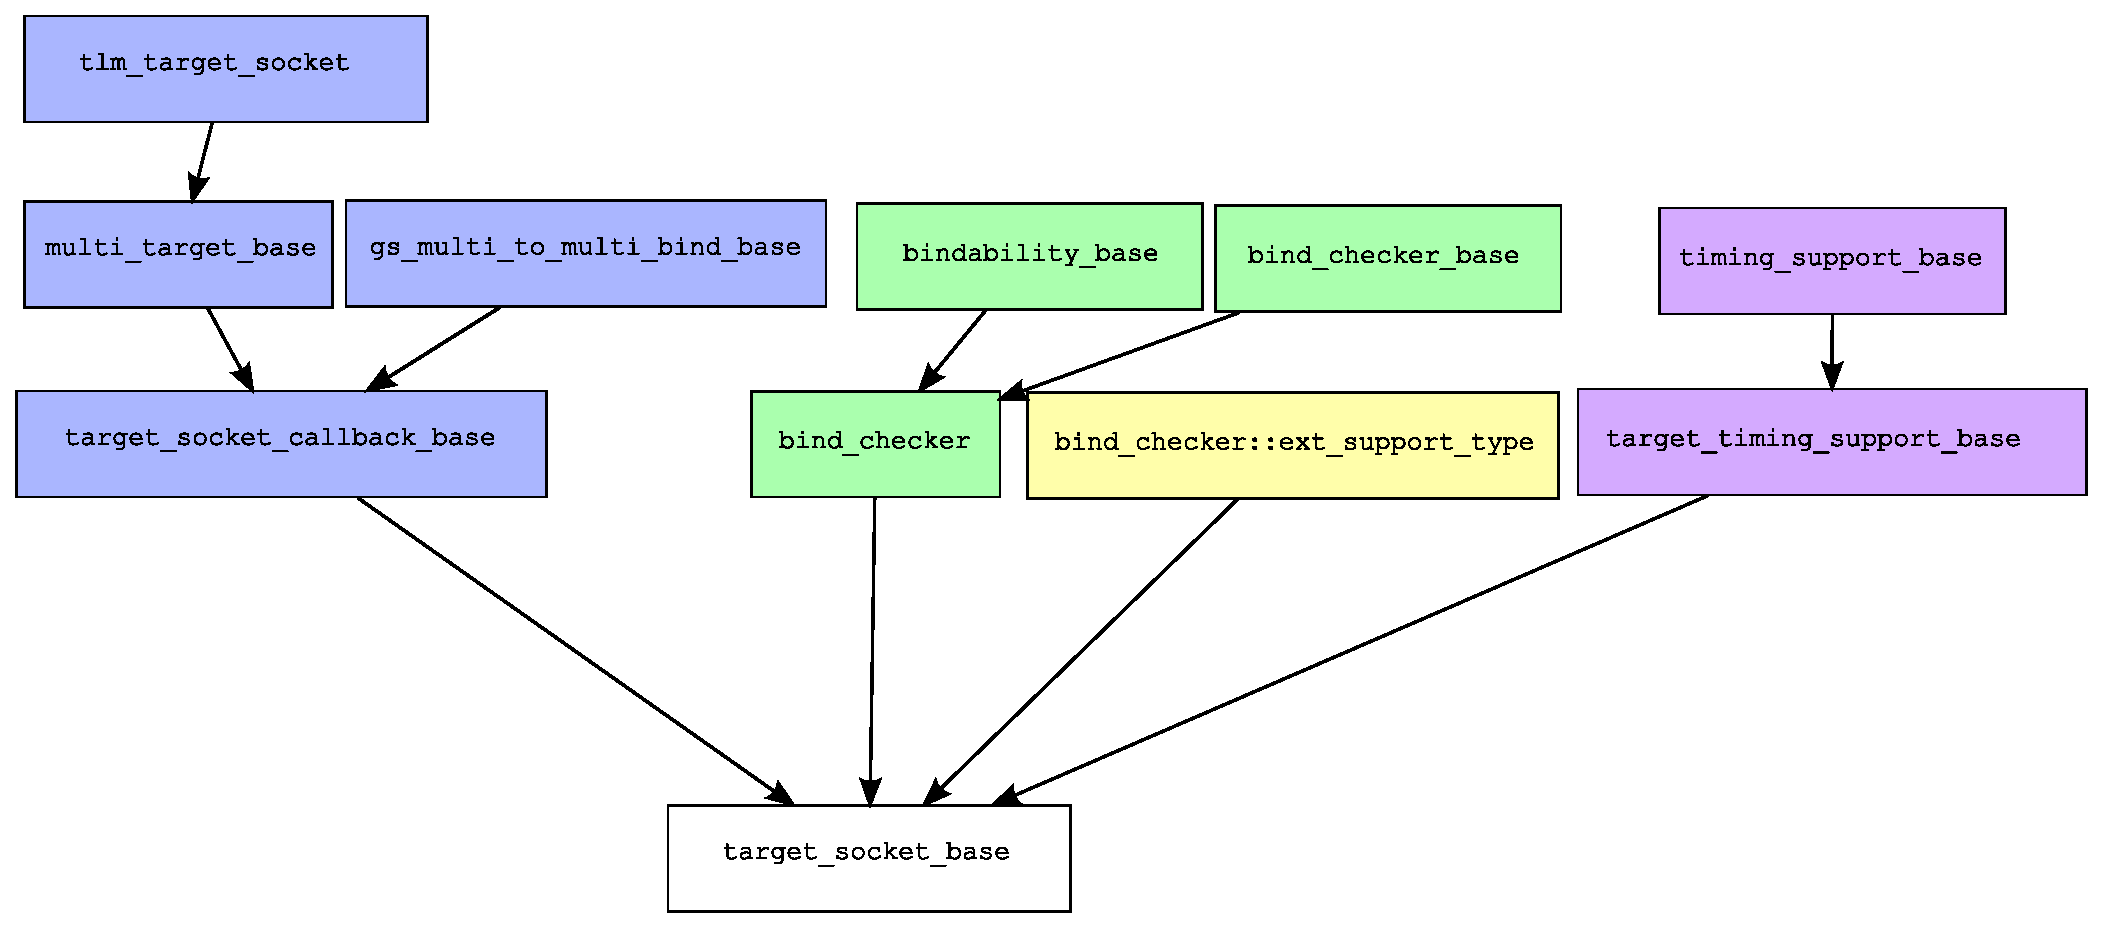
\includegraphics[scale=0.4]{tsockch}
\caption{Target Socket Class Hierarchy}
\label{fig:tsockch}
\end{center}
\end{figure}

Obviously the target socket is pretty similar to the initiator socket. It simply lacks the memory management part. The concepts used for the multi sockets that allow for sender identification, the bind check, the extension API and the timing info distribution are all the same as in the initiator socket.

Note the \code{gs\_multi\_to\_multi\_bind\_base}. Its use is explained on page 7 in connection with the \code{MULTI\_MULTI\_BASE} template argument.


\end{document}